\section{Vœux des Étudiants}
\label{sec::stud_wish}


\begin{figure}[H]
	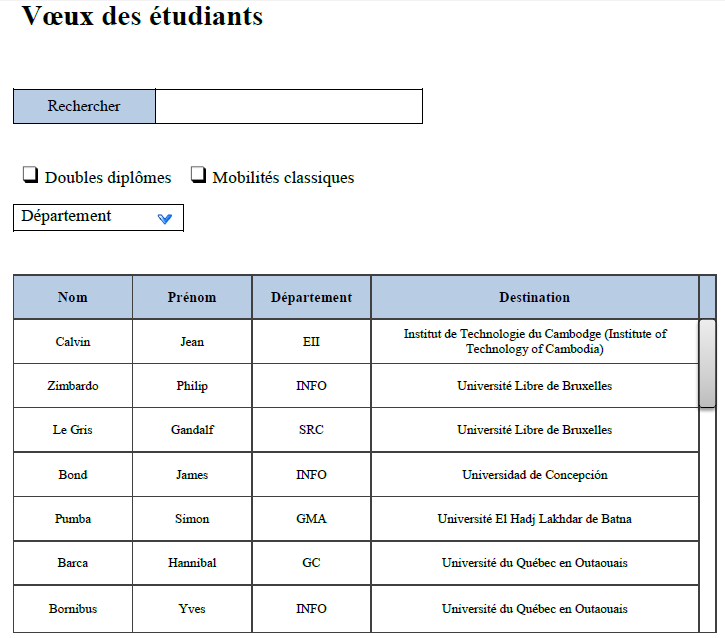
\includegraphics[scale=0.8]{Etudiant/Voeux.PNG}
	\caption{Page des vœux de tous les étudiants}
	\label{fig::list_wish}
\end{figure}


La figure \ref{fig::list_wish} représente la page permettant d'avoir accès aux vœux de tous les étudiants.

On peut filtrer cette liste avec un système de checkbox et de champs de recherche. On peut, par exemple, soit directement taper le nom de l'élève dans le champs de recherche ou bien avoir accès aux étudiants partant en double diplôme en cochant la case correspondante.

De plus chaque étudiant dans le tableau est un lien vers sa page d'accueil en lecture seule (afin empêcher quiconque de modifier les vœux des autres étudiants).

